\documentclass{beamer}
\usepackage[latin1]{inputenc}
\usepackage{xcolor}
\usepackage{hyperref}
\usepackage{minted}
\usepackage{graphicx}
\usepackage{tikz}
\usetikzlibrary{fadings}

\usetheme{default}
\usecolortheme{default}

\title{COMP3320 Introduction to OpenGL}
\author{Alex Biddulph}
\institute{
    The University of Newcastle, Australia
    \and
    Based on the work provided at \url{www.learnopengl.com}
}
\date{Semester 2, 2019}

\begin{document}

\begin{frame}
\titlepage
\end{frame}

\begin{frame}[fragile]{Vertex Attributes}
    \begin{itemize}
        \item Allows us to specify auxilliary data for each vertex
        \item Colour, texture coordinates, etc.
        \item An example specifying vertex colour information
\begin{minted}{c++}
    float vertices[] = {
        // positions         // colors
         0.5f, -0.5f, 0.0f,  1.0f, 0.0f, 0.0f,
        -0.5f, -0.5f, 0.0f,  0.0f, 1.0f, 0.0f,
         0.0f,  0.5f, 0.0f,  0.0f, 0.0f, 1.0f };
\end{minted}
        \item Must specify offset and stride for {\color{blue}\verb"glVertexAttribPointer"}
        \item[] 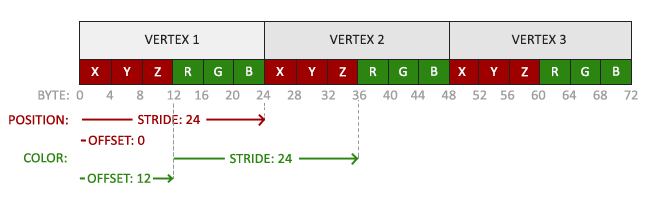
\includegraphics[width=0.90\textwidth]{images/vertex_attribute_pointer_interleaved.png}
    \end{itemize}
    {\footnotesize{Image sourced from \url{learnopengl.com/Getting-started/Shaders}}}
\end{frame}

\begin{frame}[fragile]{Vertex Attributes}
    Result should look like this
    \begin{center}
        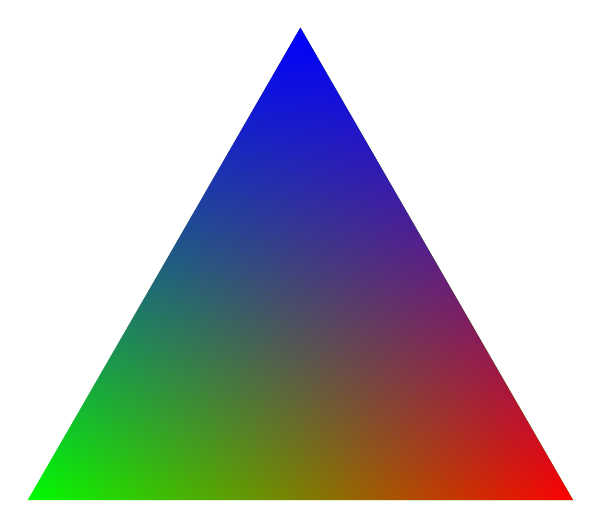
\begin{tikzpicture}
            \fill[green] (90:4) -- (210:4) -- (-30:4) -- cycle;
            \fill[red,path fading=west] (90:4) -- (210:4) -- (-30:4) -- cycle;
            \fill[blue,path fading=south] (90:4) -- (210:4) -- (-30:4) -- cycle;
        \end{tikzpicture}
    \end{center}
\end{frame}

\end{document}
